\documentclass{standalone}
\usepackage{tikz}
\usetikzlibrary{patterns, positioning}
\usepackage[sfdefault]{ClearSans} %% option 'sfdefault' activates Clear Sans as the default text font
\usepackage[T1]{fontenc}

\begin{document}
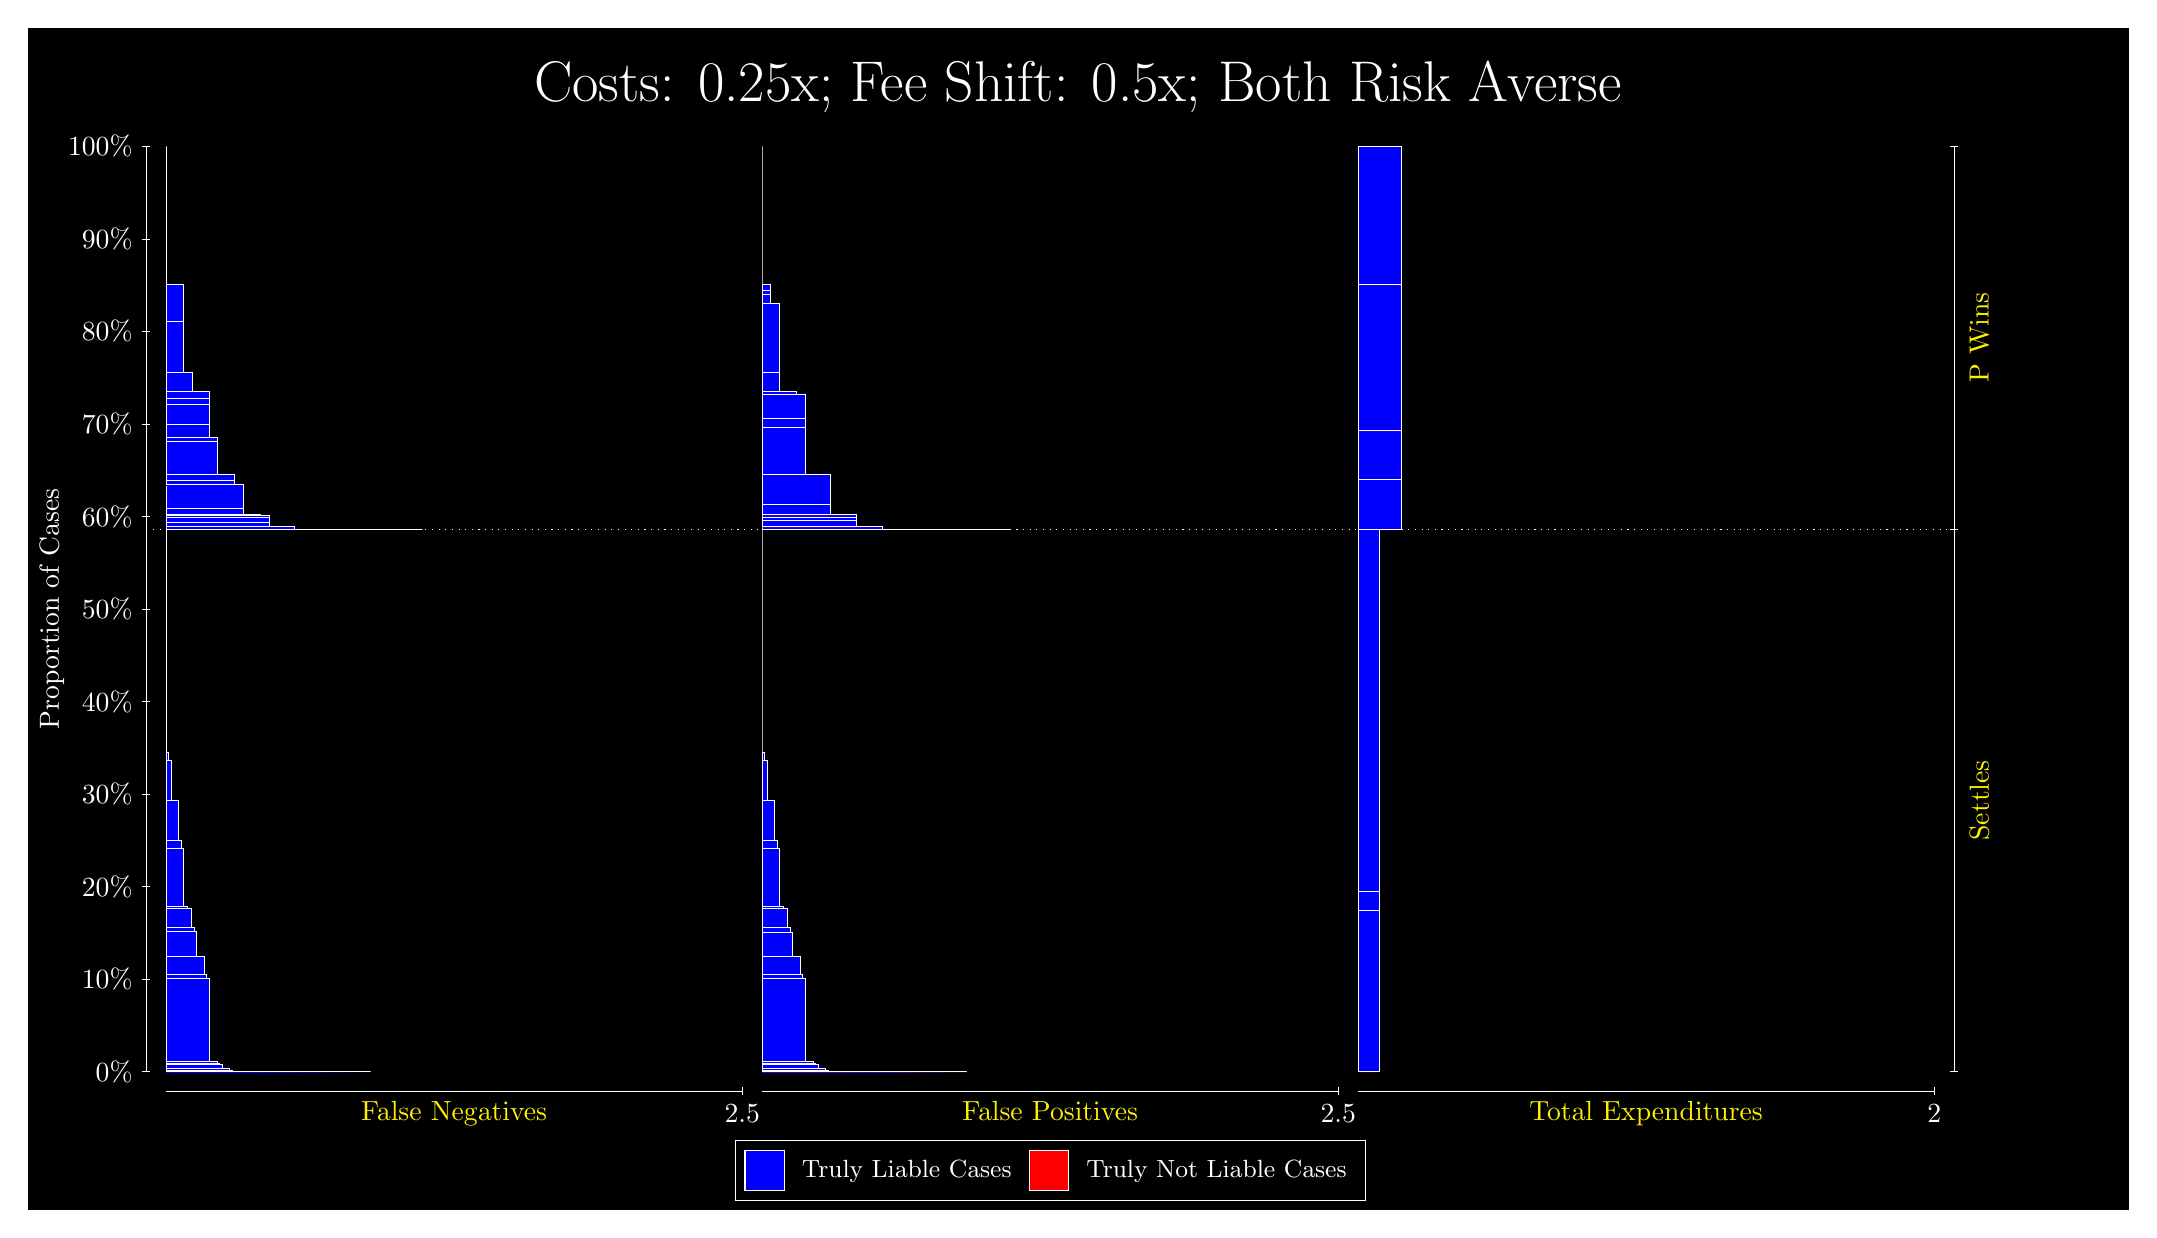
\begin{tikzpicture}
\draw[fill=black] (0,0) rectangle (26.667,15);
\draw[text=white] (0,13.5) rectangle (26.667,15) node[midway] {\huge Costs: 0.25x; Fee Shift: 0.5x; Both Risk Averse};
\draw[white, very thin] (1.5,1.75) -- (1.5,13.5);
\node[rotate=90, text=white, anchor=center] at (0.3, 7.625) {Proportion of Cases};
\draw[white, very thin] (1.45,1.75) -- (1.55,1.75);
\node[text=white, anchor=east] at (1.45, 1.75) {0\%};
\draw[white, very thin] (1.45,2.925) -- (1.55,2.925);
\node[text=white, anchor=east] at (1.45, 2.925) {10\%};
\draw[white, very thin] (1.45,4.1) -- (1.55,4.1);
\node[text=white, anchor=east] at (1.45, 4.1) {20\%};
\draw[white, very thin] (1.45,5.275) -- (1.55,5.275);
\node[text=white, anchor=east] at (1.45, 5.275) {30\%};
\draw[white, very thin] (1.45,6.45) -- (1.55,6.45);
\node[text=white, anchor=east] at (1.45, 6.45) {40\%};
\draw[white, very thin] (1.45,7.625) -- (1.55,7.625);
\node[text=white, anchor=east] at (1.45, 7.625) {50\%};
\draw[white, very thin] (1.45,8.8) -- (1.55,8.8);
\node[text=white, anchor=east] at (1.45, 8.8) {60\%};
\draw[white, very thin] (1.45,9.975) -- (1.55,9.975);
\node[text=white, anchor=east] at (1.45, 9.975) {70\%};
\draw[white, very thin] (1.45,11.15) -- (1.55,11.15);
\node[text=white, anchor=east] at (1.45, 11.15) {80\%};
\draw[white, very thin] (1.45,12.325) -- (1.55,12.325);
\node[text=white, anchor=east] at (1.45, 12.325) {90\%};
\draw[white, very thin] (1.45,13.5) -- (1.55,13.5);
\node[text=white, anchor=east] at (1.45, 13.5) {100\%};

\draw[white, very thin] (24.457,1.75) -- (24.457,13.5);
\draw[white, very thin] (24.407,1.75) -- (24.507,1.75);
\node[anchor=west] at (24.407, 1.75) {};
\draw[white, very thin] (24.407,8.6378) -- (24.507,8.6378);
\node[anchor=west] at (24.407, 8.6378) {};
\draw[white, very thin] (24.407,13.5) -- (24.507,13.5);
\node[anchor=west] at (24.407, 13.5) {};

\draw[white, very thin, fill=blue] (1.75,1.75) rectangle (4.3482,1.75);
\draw[white, very thin, fill=blue] (1.75,1.75) rectangle (4.0554,1.75);
\draw[white, very thin, fill=blue] (1.75,1.75) rectangle (4.0229,1.75);
\draw[white, very thin, fill=blue] (1.75,1.75) rectangle (3.7627,1.75);
\draw[white, very thin, fill=blue] (1.75,1.75) rectangle (3.7302,1.75);
\draw[white, very thin, fill=blue] (1.75,1.75) rectangle (3.6976,1.75);
\draw[white, very thin, fill=blue] (1.75,1.75) rectangle (3.6163,1.75);
\draw[white, very thin, fill=blue] (1.75,1.75) rectangle (3.4374,1.75);
\draw[white, very thin, fill=blue] (1.75,1.75) rectangle (3.4049,1.75);
\draw[white, very thin, fill=blue] (1.75,1.75) rectangle (3.3723,1.75);
\draw[white, very thin, fill=blue] (1.75,1.75) rectangle (3.3236,1.75);
\draw[white, very thin, fill=blue] (1.75,1.75) rectangle (3.291,1.75);
\draw[white, very thin, fill=blue] (1.75,1.75) rectangle (3.1121,1.75);
\draw[white, very thin, fill=blue] (1.75,1.75) rectangle (3.0796,1.75);
\draw[white, very thin, fill=blue] (1.75,1.75) rectangle (3.0471,1.75);
\draw[white, very thin, fill=blue] (1.75,1.75) rectangle (3.0308,1.75);
\draw[white, very thin, fill=blue] (1.75,1.75) rectangle (2.9983,1.75);
\draw[white, very thin, fill=blue] (1.75,1.75) rectangle (2.9657,1.75);
\draw[white, very thin, fill=blue] (1.75,1.75) rectangle (2.8844,1.751);
\draw[white, very thin, fill=blue] (1.75,1.751) rectangle (2.7868,1.7533);
\draw[white, very thin, fill=blue] (1.75,1.7533) rectangle (2.7543,1.7535);
\draw[white, very thin, fill=blue] (1.75,1.7535) rectangle (2.7218,1.754);
\draw[white, very thin, fill=blue] (1.75,1.754) rectangle (2.7055,1.754);
\draw[white, very thin, fill=blue] (1.75,1.754) rectangle (2.673,1.7541);
\draw[white, very thin, fill=blue] (1.75,1.7541) rectangle (2.6405,1.7541);
\draw[white, very thin, fill=blue] (1.75,1.7541) rectangle (2.5917,1.7637);
\draw[white, very thin, fill=blue] (1.75,1.7637) rectangle (2.5591,1.7909);
\draw[white, very thin, fill=blue] (1.75,1.7909) rectangle (2.4616,1.8445);
\draw[white, very thin, fill=blue] (1.75,1.8445) rectangle (2.429,1.8508);
\draw[white, very thin, fill=blue] (1.75,1.8508) rectangle (2.3965,1.875);
\draw[white, very thin, fill=blue] (1.75,1.875) rectangle (2.3802,1.8751);
\draw[white, very thin, fill=blue] (1.75,1.8751) rectangle (2.3477,1.8796);
\draw[white, very thin, fill=blue] (1.75,1.8796) rectangle (2.3152,1.8797);
\draw[white, very thin, fill=blue] (1.75,1.8797) rectangle (2.2989,2.9317);
\draw[white, very thin, fill=blue] (1.75,2.9317) rectangle (2.2664,2.988);
\draw[white, very thin, fill=blue] (1.75,2.988) rectangle (2.2339,3.2171);
\draw[white, very thin, fill=blue] (1.75,3.2171) rectangle (2.1363,3.5249);
\draw[white, very thin, fill=blue] (1.75,3.5249) rectangle (2.1037,3.5785);
\draw[white, very thin, fill=blue] (1.75,3.5785) rectangle (2.0712,3.825);
\draw[white, very thin, fill=blue] (1.75,3.825) rectangle (2.055,3.8255);
\draw[white, very thin, fill=blue] (1.75,3.8255) rectangle (2.0224,3.8491);
\draw[white, very thin, fill=blue] (1.75,3.8491) rectangle (1.9899,3.8496);
\draw[white, very thin, fill=blue] (1.75,3.8496) rectangle (1.9736,4.5798);
\draw[white, very thin, fill=blue] (1.75,4.5798) rectangle (1.9411,4.6907);
\draw[white, very thin, fill=blue] (1.75,4.6907) rectangle (1.9086,5.1939);
\draw[white, very thin, fill=blue] (1.75,5.1939) rectangle (1.811,5.6971);
\draw[white, very thin, fill=blue] (1.75,5.6971) rectangle (1.7785,5.808);
\draw[white, very thin, fill=red] (1.75,5.808) rectangle (1.75,5.808);
\draw[white, very thin, fill=blue] (1.75,5.808) rectangle (1.75,8.6378);
\draw[white, very thin, fill=blue] (1.75,8.6378) rectangle (5.0069,8.6378);
\draw[white, very thin, fill=blue] (1.75,8.6378) rectangle (4.6816,8.6378);
\draw[white, very thin, fill=blue] (1.75,8.6378) rectangle (4.3563,8.6378);
\draw[white, very thin, fill=blue] (1.75,8.6378) rectangle (4.2465,8.6378);
\draw[white, very thin, fill=blue] (1.75,8.6378) rectangle (4.031,8.6379);
\draw[white, very thin, fill=blue] (1.75,8.6379) rectangle (4.031,8.638);
\draw[white, very thin, fill=blue] (1.75,8.638) rectangle (3.9213,8.638);
\draw[white, very thin, fill=blue] (1.75,8.638) rectangle (3.7058,8.6399);
\draw[white, very thin, fill=blue] (1.75,8.6399) rectangle (3.7058,8.6412);
\draw[white, very thin, fill=blue] (1.75,8.6412) rectangle (3.596,8.6412);
\draw[white, very thin, fill=blue] (1.75,8.6412) rectangle (3.3805,8.6697);
\draw[white, very thin, fill=blue] (1.75,8.6697) rectangle (3.2707,8.6697);
\draw[white, very thin, fill=blue] (1.75,8.6697) rectangle (3.2707,8.6698);
\draw[white, very thin, fill=blue] (1.75,8.6698) rectangle (3.0552,8.7196);
\draw[white, very thin, fill=blue] (1.75,8.7196) rectangle (3.0552,8.7944);
\draw[white, very thin, fill=blue] (1.75,8.7944) rectangle (3.0552,8.8103);
\draw[white, very thin, fill=blue] (1.75,8.8103) rectangle (2.9454,8.8137);
\draw[white, very thin, fill=blue] (1.75,8.8137) rectangle (2.9454,8.8205);
\draw[white, very thin, fill=blue] (1.75,8.8205) rectangle (2.9454,8.8209);
\draw[white, very thin, fill=blue] (1.75,8.8209) rectangle (2.7299,8.9069);
\draw[white, very thin, fill=blue] (1.75,8.9069) rectangle (2.7299,9.204);
\draw[white, very thin, fill=blue] (1.75,9.204) rectangle (2.6201,9.2048);
\draw[white, very thin, fill=blue] (1.75,9.2048) rectangle (2.6201,9.263);
\draw[white, very thin, fill=blue] (1.75,9.263) rectangle (2.6201,9.3304);
\draw[white, very thin, fill=blue] (1.75,9.3304) rectangle (2.4046,9.3354);
\draw[white, very thin, fill=blue] (1.75,9.3354) rectangle (2.4046,9.7577);
\draw[white, very thin, fill=blue] (1.75,9.7577) rectangle (2.4046,9.8059);
\draw[white, very thin, fill=blue] (1.75,9.8059) rectangle (2.2948,9.966);
\draw[white, very thin, fill=blue] (1.75,9.966) rectangle (2.2948,10.222);
\draw[white, very thin, fill=blue] (1.75,10.222) rectangle (2.2948,10.299);
\draw[white, very thin, fill=blue] (1.75,10.299) rectangle (2.2948,10.39);
\draw[white, very thin, fill=blue] (1.75,10.39) rectangle (2.0793,10.627);
\draw[white, very thin, fill=blue] (1.75,10.627) rectangle (1.9696,11.273);
\draw[white, very thin, fill=blue] (1.75,11.273) rectangle (1.9696,11.748);
\draw[white, very thin, fill=blue] (1.75,11.748) rectangle (1.7541,11.791);
\draw[white, very thin, fill=blue] (1.75,11.791) rectangle (1.7541,11.791);
\draw[white, very thin, fill=red] (1.75,11.791) rectangle (1.75,11.791);
\draw[white, very thin, fill=blue] (1.75,11.791) rectangle (1.75,13.5);
\draw[white, very thin, fill=red] (9.3189,1.75) rectangle (11.917,1.75);
\draw[white, very thin, fill=blue] (9.3189,1.75) rectangle (11.917,1.75);
\draw[white, very thin, fill=red] (9.3189,1.75) rectangle (11.624,1.75);
\draw[white, very thin, fill=blue] (9.3189,1.75) rectangle (11.624,1.75);
\draw[white, very thin, fill=blue] (9.3189,1.75) rectangle (11.592,1.75);
\draw[white, very thin, fill=red] (9.3189,1.75) rectangle (11.332,1.75);
\draw[white, very thin, fill=blue] (9.3189,1.75) rectangle (11.332,1.75);
\draw[white, very thin, fill=blue] (9.3189,1.75) rectangle (11.299,1.75);
\draw[white, very thin, fill=blue] (9.3189,1.75) rectangle (11.266,1.75);
\draw[white, very thin, fill=red] (9.3189,1.75) rectangle (11.185,1.75);
\draw[white, very thin, fill=blue] (9.3189,1.75) rectangle (11.185,1.75);
\draw[white, very thin, fill=blue] (9.3189,1.75) rectangle (11.006,1.75);
\draw[white, very thin, fill=blue] (9.3189,1.75) rectangle (10.974,1.75);
\draw[white, very thin, fill=blue] (9.3189,1.75) rectangle (10.941,1.75);
\draw[white, very thin, fill=red] (9.3189,1.75) rectangle (10.892,1.75);
\draw[white, very thin, fill=blue] (9.3189,1.75) rectangle (10.892,1.75);
\draw[white, very thin, fill=blue] (9.3189,1.75) rectangle (10.86,1.75);
\draw[white, very thin, fill=blue] (9.3189,1.75) rectangle (10.681,1.75);
\draw[white, very thin, fill=blue] (9.3189,1.75) rectangle (10.648,1.75);
\draw[white, very thin, fill=blue] (9.3189,1.75) rectangle (10.616,1.75);
\draw[white, very thin, fill=red] (9.3189,1.75) rectangle (10.6,1.75);
\draw[white, very thin, fill=blue] (9.3189,1.75) rectangle (10.6,1.75);
\draw[white, very thin, fill=blue] (9.3189,1.75) rectangle (10.567,1.75);
\draw[white, very thin, fill=blue] (9.3189,1.75) rectangle (10.535,1.75);
\draw[white, very thin, fill=red] (9.3189,1.75) rectangle (10.453,1.75);
\draw[white, very thin, fill=blue] (9.3189,1.75) rectangle (10.453,1.751);
\draw[white, very thin, fill=blue] (9.3189,1.751) rectangle (10.356,1.7533);
\draw[white, very thin, fill=blue] (9.3189,1.7533) rectangle (10.323,1.7535);
\draw[white, very thin, fill=blue] (9.3189,1.7535) rectangle (10.291,1.754);
\draw[white, very thin, fill=blue] (9.3189,1.754) rectangle (10.274,1.754);
\draw[white, very thin, fill=blue] (9.3189,1.754) rectangle (10.242,1.7541);
\draw[white, very thin, fill=blue] (9.3189,1.7541) rectangle (10.209,1.7541);
\draw[white, very thin, fill=red] (9.3189,1.7541) rectangle (10.161,1.7541);
\draw[white, very thin, fill=blue] (9.3189,1.7541) rectangle (10.161,1.7637);
\draw[white, very thin, fill=blue] (9.3189,1.7637) rectangle (10.128,1.7909);
\draw[white, very thin, fill=blue] (9.3189,1.7909) rectangle (10.03,1.8445);
\draw[white, very thin, fill=blue] (9.3189,1.8445) rectangle (9.9979,1.8508);
\draw[white, very thin, fill=blue] (9.3189,1.8508) rectangle (9.9654,1.875);
\draw[white, very thin, fill=blue] (9.3189,1.875) rectangle (9.9491,1.8751);
\draw[white, very thin, fill=blue] (9.3189,1.8751) rectangle (9.9166,1.8796);
\draw[white, very thin, fill=blue] (9.3189,1.8796) rectangle (9.884,1.8797);
\draw[white, very thin, fill=red] (9.3189,1.8797) rectangle (9.8678,1.8797);
\draw[white, very thin, fill=blue] (9.3189,1.8797) rectangle (9.8678,2.9316);
\draw[white, very thin, fill=blue] (9.3189,2.9316) rectangle (9.8353,2.9879);
\draw[white, very thin, fill=blue] (9.3189,2.9879) rectangle (9.8027,3.2171);
\draw[white, very thin, fill=blue] (9.3189,3.2171) rectangle (9.7051,3.5248);
\draw[white, very thin, fill=blue] (9.3189,3.5248) rectangle (9.6726,3.5784);
\draw[white, very thin, fill=blue] (9.3189,3.5784) rectangle (9.6401,3.8249);
\draw[white, very thin, fill=blue] (9.3189,3.8249) rectangle (9.6238,3.8254);
\draw[white, very thin, fill=blue] (9.3189,3.8254) rectangle (9.5913,3.8491);
\draw[white, very thin, fill=blue] (9.3189,3.8491) rectangle (9.5588,3.8496);
\draw[white, very thin, fill=blue] (9.3189,3.8496) rectangle (9.5425,4.5798);
\draw[white, very thin, fill=blue] (9.3189,4.5798) rectangle (9.51,4.6907);
\draw[white, very thin, fill=blue] (9.3189,4.6907) rectangle (9.4774,5.1939);
\draw[white, very thin, fill=blue] (9.3189,5.1939) rectangle (9.3799,5.697);
\draw[white, very thin, fill=blue] (9.3189,5.697) rectangle (9.3473,5.8079);
\draw[white, very thin, fill=blue] (9.3189,5.8079) rectangle (9.3189,8.6378);
\draw[white, very thin, fill=red] (9.3189,8.6378) rectangle (12.466,8.6378);
\draw[white, very thin, fill=blue] (9.3189,8.6378) rectangle (12.466,8.6378);
\draw[white, very thin, fill=red] (9.3189,8.6378) rectangle (12.141,8.6378);
\draw[white, very thin, fill=blue] (9.3189,8.6378) rectangle (12.141,8.6378);
\draw[white, very thin, fill=red] (9.3189,8.6378) rectangle (11.815,8.6378);
\draw[white, very thin, fill=blue] (9.3189,8.6378) rectangle (11.815,8.6378);
\draw[white, very thin, fill=blue] (9.3189,8.6378) rectangle (11.815,8.6378);
\draw[white, very thin, fill=blue] (9.3189,8.6378) rectangle (11.49,8.6379);
\draw[white, very thin, fill=red] (9.3189,8.6379) rectangle (11.49,8.6379);
\draw[white, very thin, fill=blue] (9.3189,8.6379) rectangle (11.49,8.638);
\draw[white, very thin, fill=red] (9.3189,8.638) rectangle (11.165,8.638);
\draw[white, very thin, fill=blue] (9.3189,8.638) rectangle (11.165,8.6412);
\draw[white, very thin, fill=red] (9.3189,8.6412) rectangle (11.055,8.6412);
\draw[white, very thin, fill=blue] (9.3189,8.6412) rectangle (11.055,8.6412);
\draw[white, very thin, fill=red] (9.3189,8.6412) rectangle (10.84,8.6412);
\draw[white, very thin, fill=blue] (9.3189,8.6412) rectangle (10.84,8.6698);
\draw[white, very thin, fill=blue] (9.3189,8.6698) rectangle (10.73,8.6698);
\draw[white, very thin, fill=red] (9.3189,8.6698) rectangle (10.73,8.6698);
\draw[white, very thin, fill=blue] (9.3189,8.6698) rectangle (10.73,8.6698);
\draw[white, very thin, fill=red] (9.3189,8.6698) rectangle (10.514,8.6698);
\draw[white, very thin, fill=blue] (9.3189,8.6698) rectangle (10.514,8.7523);
\draw[white, very thin, fill=blue] (9.3189,8.7523) rectangle (10.514,8.7911);
\draw[white, very thin, fill=blue] (9.3189,8.7911) rectangle (10.514,8.8209);
\draw[white, very thin, fill=blue] (9.3189,8.8209) rectangle (10.404,8.8209);
\draw[white, very thin, fill=red] (9.3189,8.8209) rectangle (10.404,8.8209);
\draw[white, very thin, fill=blue] (9.3189,8.8209) rectangle (10.404,8.8209);
\draw[white, very thin, fill=red] (9.3189,8.8209) rectangle (10.189,8.8209);
\draw[white, very thin, fill=blue] (9.3189,8.8209) rectangle (10.189,8.9539);
\draw[white, very thin, fill=blue] (9.3189,8.9539) rectangle (10.189,9.3303);
\draw[white, very thin, fill=blue] (9.3189,9.3303) rectangle (10.079,9.3303);
\draw[white, very thin, fill=red] (9.3189,9.3303) rectangle (10.079,9.3303);
\draw[white, very thin, fill=blue] (9.3189,9.3303) rectangle (10.079,9.3304);
\draw[white, very thin, fill=blue] (9.3189,9.3304) rectangle (9.8637,9.926);
\draw[white, very thin, fill=blue] (9.3189,9.926) rectangle (9.8637,10.051);
\draw[white, very thin, fill=blue] (9.3189,10.051) rectangle (9.8637,10.346);
\draw[white, very thin, fill=blue] (9.3189,10.346) rectangle (9.7539,10.346);
\draw[white, very thin, fill=red] (9.3189,10.346) rectangle (9.7539,10.346);
\draw[white, very thin, fill=blue] (9.3189,10.346) rectangle (9.7539,10.384);
\draw[white, very thin, fill=blue] (9.3189,10.384) rectangle (9.7539,10.39);
\draw[white, very thin, fill=blue] (9.3189,10.39) rectangle (9.5384,10.633);
\draw[white, very thin, fill=blue] (9.3189,10.633) rectangle (9.5384,11.511);
\draw[white, very thin, fill=blue] (9.3189,11.511) rectangle (9.4287,11.623);
\draw[white, very thin, fill=red] (9.3189,11.623) rectangle (9.4287,11.623);
\draw[white, very thin, fill=blue] (9.3189,11.623) rectangle (9.4287,11.67);
\draw[white, very thin, fill=blue] (9.3189,11.67) rectangle (9.4287,11.748);
\draw[white, very thin, fill=blue] (9.3189,11.748) rectangle (9.3189,13.5);
\draw[white, very thin, fill=red] (16.888,1.75) rectangle (17.162,1.75);
\draw[white, very thin, fill=blue] (16.888,1.75) rectangle (17.162,3.8032);
\draw[white, very thin, fill=red] (16.888,3.8032) rectangle (17.162,3.8032);
\draw[white, very thin, fill=blue] (16.888,3.8032) rectangle (17.162,4.0401);
\draw[white, very thin, fill=red] (16.888,4.0401) rectangle (17.162,4.0401);
\draw[white, very thin, fill=blue] (16.888,4.0401) rectangle (17.162,8.6378);
\draw[white, very thin, fill=red] (16.888,8.6378) rectangle (17.437,8.6378);
\draw[white, very thin, fill=blue] (16.888,8.6378) rectangle (17.437,9.269);
\draw[white, very thin, fill=red] (16.888,9.269) rectangle (17.437,9.269);
\draw[white, very thin, fill=blue] (16.888,9.269) rectangle (17.437,9.8876);
\draw[white, very thin, fill=red] (16.888,9.8876) rectangle (17.437,9.8876);
\draw[white, very thin, fill=blue] (16.888,9.8876) rectangle (17.437,11.743);
\draw[white, very thin, fill=red] (16.888,11.743) rectangle (17.437,11.743);
\draw[white, very thin, fill=blue] (16.888,11.743) rectangle (17.437,13.5);
\draw[white, dotted] (1.5,8.6378) -- (24.457,8.6378);
\draw[white, very thin] (1.75,1.5) -- (9.0689,1.5);
\node[text=yellow, anchor=north] at (5.4094, 1.5) {False Negatives};
\draw[white, very thin] (9.0689,1.45) -- (9.0689,1.55);
\node[text=white, anchor=north] at (9.0689, 1.45) {2.5};

\draw[white, very thin] (9.3189,1.5) -- (16.638,1.5);
\node[text=yellow, anchor=north] at (12.978, 1.5) {False Positives};
\draw[white, very thin] (16.638,1.45) -- (16.638,1.55);
\node[text=white, anchor=north] at (16.638, 1.45) {2.5};

\draw[white, very thin] (16.888,1.5) -- (24.207,1.5);
\node[text=yellow, anchor=north] at (20.547, 1.5) {Total Expenditures};
\draw[white, very thin] (24.207,1.45) -- (24.207,1.55);
\node[text=white, anchor=north] at (24.207, 1.45) {2};

\node[text=yellow, centered, rotate=90] at (24.777, 5.1939) {Settles};
\node[text=yellow, centered, rotate=90] at (24.777, 11.069) {P Wins};

\draw (12.978300999999998,1.5) node[draw=none] (baseCoordinate) {};
\begin{scope}[align=center]
        \matrix[scale=0.5, draw=white, below=0.5cm of baseCoordinate, nodes={draw}, column sep=0.1cm]{
            \node[rectangle, draw, minimum width=0.5cm, minimum height=0.5cm, fill=blue] {}; &
            \node[draw=none, font=\small, text=white] (B) {Truly Liable Cases}; &
            \node[rectangle, draw, minimum width=0.5cm, minimum height=0.5cm, fill=red] {}; &
            \node[draw=none, font=\small, text=white] (B) {Truly Not Liable Cases}; \\
            };
\end{scope}

\end{tikzpicture}
\end{document}